\chapter{XML protokol}
\label{kap_xml}
Pan Ing. Peter Macejko ve své diplomové práci navrh systém vzdálené správy strojů pomocí komunikačního protokolu, využívajícího XML. V této kapitole budou shrnuty všechny 
navržené postupy od mapování SNMP informačního modelu až, po komunikační struktury využívané správcem a spravovanými zařízeními.

\section{Obecný informační model}
Informační model je nedílnou součástí celého systému správy dat. Do něj jsou mapována veškerá monitorovaná data a jsou zde i vyjádřeny vztahy mezi daty. Ve skutečnosti
omezuje počet a druh možných dotazů. Výsledný systém, který byl pro popis jednotlivých zařízení navrženi, vychází z několika různých přístupů abstrakce a popisu dat.

Nejprve byla analýza problému založena na dvou možnostech - přímém mapování MIB stromu do XML dokumentu, kdy by jednotlivé uzly přesně odpovídaly MIB struktuře; objektově
orientovaném využívajícím objektové paradigma. První přístup má výhodu ve snadném převodu MIB databáze do nového formátu, ale naopak ztrácí výhodu snadné rozšiřitelnosti,
která je vlastní XML technolgoii. Problém objektového mapování je nejednoznačné rozmístění uzlů ve stromu na objekty. Takovéto mapování by bylo nutno provádět
neautomatizovaně, tj. za asistence člověka.

Výsledkem analýzy problému je systém využívající kousek od obou přístupů. Na nejvyšší úrovni abstrakce je každé zařízení složeno z modulů. Každý modul obsahuje jistou
funkcionalitu, která je úplně oddělena od těch zbývajících. Mezi tyto moduly patří i v této práci navrhovaná brána, která propojuje zařízení bez XML podpory s ostatními
částmi sítě. V této chvíli se jedná pouze o obecný návrh každého zařízení.

\subsection{Odvození typů}
Odvozování typů je založeno na principu dědičnosti. Definice jako takové jdou od abstraktního až po detailní popis.

\subsection{Definice modulů}
Jak již bylo řečeno, každé zařízení se skládá z modulů. Jednotlivé moduly jsou též popsány XML schématem. Každé takové schéma
musí splňovat přesné požadavky na poskytované informace.

Musí být detailně popsána funkčnost, přiděleno unikátní jméno, typ a cesta ve stromové struktuře, použitá pro adresaci jednotlivých uzlů. 
SNMP moduly mají definován kořenový element, který je využit pro spojování více MIB informačních bází dohromady.

Přesný popis je možné nalézt v \cite{macejko_dipl} v kapitole 5.2.3.

\subsection{Popis zařízení}
Pro popis zařízení je využito XML schéma, stejně jako pro popis dalších částí (modulů apod.). Na obrázku \ref{obr_xml_popis_zarizeni} je znázorněno,
jak vypadá zařízení popsané od nejvyšší úrovně. 

\begin{figure}[htp]
	\begin{center}
		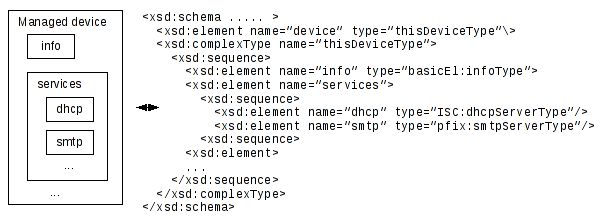
\includegraphics[width=15cm]{obrazky/03_popis_zarizeni.png}
		\caption{Popis zařízení v XML schématu (\cite{macejko_dipl})}
		\label{obr_xml_popis_zarizeni}
	\end{center}
\end{figure}

\subsection{Oznamovací zprávy}
Oznámení jsou takové zprávy, které jsou zasílány manažerovi v případě, že se na monitorovaném zařízení vyskytne nějaká událost (shodné s SNMP Trap zprávami).
V rámci SNMP jsou tyto zprávy součástí datového modelu, nicméně tyto specifické uzly MIB stromu nenesou žádná data, a jsou tudíž použité pouze při generování typu
chyby či události. 

V navrženém systému jsou všechna možné upozornění (ať již předdefinované, či definované administrátorem) umístěny ve speciálním uzlu stromu \verb|notifications|, 
kde je velice jednoduché dohledat, jaké události mohou způsobit zaslání oznamuvací zprávy. Každý modul pak může mít specifikován speciální typ \verb|NotificationType|,
který popisuje právě onu událost.

\subsection{Adresace dat}
Pro adresaci dat je možno využít postupů XPath a XQuery. Jednotlivými výrazy ať už v jednom či druhém případě se bude manažer dotazovat na jednotlivé uzly v
rámci spravované databáze.


\section{Mapování MIB do XML}
V předchozí části byl rozebrán čistě obecný model popisu zařízení. Pro monitorované stroje, které nejsou kompatibilní s XML protokolem, musí existovat brána,
která bude překládat dotazy z jednoho protokolu na druhý a stejně tak i odpovědi. Je tedy nutné přesně definovat postup přepisu MIB na XML.

Je nutné vyřešit tři základní problémy - jak importovat jednotlivé MIB do sebe; jak předefinovat datové typy a jak konvertovat celý MIB strom.

\subsection{Importy}
V rámci jednotlivých MIB jsou časté odkazy na báze vyšší úrovně, kdy pak na nižších úrovních definujeme jenom část podstromu. V rámci XML budou definovány 
odkazy jako prostory jmen, které jsou odvozeny od názvu daného MIB. Odkaz na jiné schéma bude proveden použitím odkazů na typ s příslušným názvem prostoru jmen. 

\subsection{Datové typy}
V SNMP, jak bylo řečeno v předchozí kapitole, existuje několik druhů datových typů. Jednoduché (integer, string,...), aplikačně rozšířené (Gauge, IpAddress,...) a 
uživatelem definované.

Jednoduché typy budou mapovány na jejich XML ekvivalent. Na obrázku \ref{obr_xml_smi1_typy} je soupis všech aplikačně rozšířených typů a jejich popis
pomocí XML schématu (v rámci standardu SMIv1).

\begin{figure}[htp]
	\begin{center}
		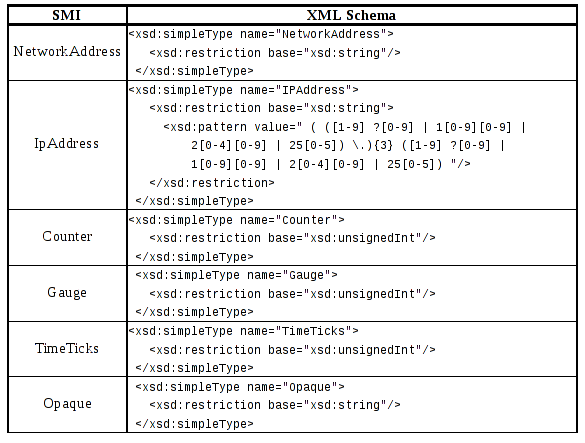
\includegraphics{obrazky/03_mapovani_smiv1.png}
		\caption{Mapování aplikačních typů SMIv1 do XML schématu (\cite{macejko_dipl})}
		\label{obr_xml_smi1_typy}
	\end{center}
\end{figure}

\begin{table}
	\centering
	{\footnotesize
	  \begin{tabular}{|p{15cm}|}
      \hline
\begin{verbatim}...
    <xsd:element name="NodeName" type="MIBName:NodeNameType"/>
...
<xsd:simpleType name="NodeNameType">
  <xsd:annotation>
    <xsd:documentation xml:lang="en">DescrText</xsd:documentation>
    <xsd:appinfo>
      <status>StatusType</status>
      <access>AccessType</access>
      <oid>AbsoluteOID</oid>
    </xsd:appinfo>
  </xsd:annotation>
  <xsd:restriction base="NodeType"/>
</xsd:simpleType>\end{verbatim}\\
      \hline
    \end{tabular}
  }
	\caption{Mapování makra OBJECT-TYPE, jednoduchý typ (SMIv1) (\cite{macejko_dipl})}
	\label{tab_xml_smi1_simple_type}
\end{table}

Součástí SMI je i možnost definovat vlastní typy. I pro tyto případy je nutno uvést definici překladu. Existují tři základní omezení při vytváření vlastních typů -
výčet, délka řetězce a rozmezí hodnot. Všechny tyto typy jsou detailně popsány a vyobrazeny v \cite{macejko_dipl}, kapitola 5.3.1.

\subsection{MIB strom}
Navržený systém využívá při mapování celého stromu oddělení definicí typů od samotné struktury stromu. Typy jsou definovány globálně a zároveň separátně od 
struktury a to z důvodu možného použití typů v rámci jiného modulu a zároveň při omezení přístupových práv do dané oblasti stromu. V MIB jsou objekty
definovány makry (specifikované v SMI), které popisují několik základních typů uzlů. SMIv1 specifikuje OBJECT-TYPE a TRAP-TYPE makra.

OBJECT-TYPE makro definuje uzel, který obsahuje nějaká data. Může to být samotná hodnota, položka, nebo celá řádka tabulky. Mapování pak závisí na
položce \verb|SyntaxType| v samotné definici makra.

Pakliže je hodnota položky základním, rozšířeným či uživatelsky definovaným typem, bude vytvořena globální definice typu a položka bude tvořena elementem
s jednoduchým typem. Schematicky vyjádřeno v tabulce \ref{tab_xml_smi1_simple_type}.

Jestli bude hodnotou \verb|SEQUENCE|, bude vytvořen "řádkový" typ (tabulka \ref{tab_xml_smi1_sequence}).

Hodnota \verb|SEQUENCE OF| pak vyjadřuje množinu řádkových typů (tabulka \ref{tab_xml_smi1_sequenceof}).


\begin{table}
	\centering
	{\footnotesize
	  \begin{tabular}{|p{15cm}|}
      \hline
\begin{verbatim}...
    <xsd:element minOccurs="0" maxOccurs="unbounded"
             name="NodeName" type="MIBName:NodeNameType"/>
...
<xsd:complexType name="NodeNameType">
  <xsd:sequence>
    <xsd:element name="..child.." type="..childType.."/>
    ...
  </xsd:sequence>
</xsd:complexType>\end{verbatim}\\
      \hline
    \end{tabular}
  }
	\caption{Mapování SEQUENCE, makro OBJECT-TYPE (\cite{macejko_dipl})}
	\label{tab_xml_smi1_sequence}
\end{table}

\begin{table}
	\centering
	{\footnotesize
	  \begin{tabular}{|p{15cm}|}
      \hline
\begin{verbatim}...
  <xsd:element name="atTable">
    <xsd:complexType>
      <xsd:sequence>
        <xsd:element ..SEQUENCE.. />
      </xsd:sequence>
    </xsd:complexType>
  </xsd:element>
...\end{verbatim}\\
      \hline
    \end{tabular}
  }
	\caption{Mapování SEQUENCE OF, makro OBJECT-TYPE (\cite{macejko_dipl})}
	\label{tab_xml_smi1_sequenceof}
\end{table}

Dalším typem objektu jsou upozornění definované pomocí TRAP-TYPE makra. Tyto definují uzly bez hodnot, pouze specifikují danou událost. V navrženém systému
tedy nemusí být součástí stromu, ale pouze globálních typových definicí. Bude použit jednoduchý typ popisující čas a den (datetime type) se speciálním elementem
v části \verb|appinfo|.

\begin{table}
	\centering
	{\footnotesize
	  \begin{tabular}{|p{15cm}|}
      \hline
\begin{verbatim}<xsd:simpleType name="NodeNameType">
  <xsd:annotation>
    <xsd:documentation xml:lang="en">DescrText</xsd:documentation>
    <xsd:appinfo>
      <enterprise>EnterpriseName</enterprise>
      <variable>VariableType</variable>
      <reference>ReferenceType</reference>
      <trapNumber>TrapNumber</trapNumber>
    </xsd:appinfo>
  </xsd:annotation>
  <xsd:restriction base="xsd:dateTime"/>
</xsd:simpleType>\end{verbatim}\\
      \hline
    \end{tabular}
  }
	\caption{Mapování TRAP-TYPE makra (\cite{macejko_dipl})}
	\label{tab_xml_trap_type}
\end{table}

\newpage

\section{Zprávy}
Navrhovaný systém by měl využívat spolehlivého a potvrzovaného přenosového protokolu, na rozdíl od nepotvrzovaného SNMP. Zaroveň by mělo být možno
přenášet zprávy v co nejjednodušším formátu. Proto bylo rozhodnuto o použití protokolu HTTP, který využívá přenosový protokol TCP, čímž je zajištěn 
spolehlivý přenos. Všecha data se budou přenášet pomocí HTTP zprávy POST.

HTTP je bezestavový protokol. Veškerá komunikace se sestává z dvojice dotaz a odpověď. Na serveru se neudržují jakékoliv další informace ohledně probíhajícího
spojení. Tato nenáročnost dovoluje implementaci na velice různorodém hardwaru.

Bezpečnost přenosu může být řešena za použití tunelování paketů (IPSec, STunel,...), nebo je možno využít výhody HTTPS (HTTP over SSL). 

Veškerá přenášená data budou ve formátu XML dokumentu s kořenovým uzlem \verb|message|. Tento uzel má několik atributů, které specifikují jeho zpracování a přístupová
práva. Jsou to \verb|queue|, \verb|password|, \verb|context|. První atribut určuje frontu (může být založeno na prioritním zpracování), ve které bude požadavek zpracován.
V principu ale nejsou agenti ani brány povinni takovouto funkčnost implementovat. Zprávy pak budou zpracovány sekvenčně a odpovědi budou generovány v přesném pořadí tak, 
jak přišly dotazy. Zbylé dva atributy slouží pro vymezení přístupu uživatele (\verb|context|) na určitý podstrom dat. 

Bylo již naznačeno, že zpráva může obsahovat několik jednotlivých dotazů. Struktura zprávy je vyjádřena na obrázku \ref{obr_xml_struktura_zpravy}.

\begin{figure}[htp]
	\begin{center}
		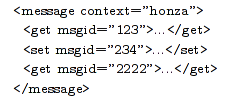
\includegraphics{obrazky/03_struktura_zpravy.png}
		\caption{Struktura XML zprávy}
		\label{obr_xml_struktura_zpravy}
	\end{center}
\end{figure}

Dotazy a odpovědi, které definují komunikaci mezi manažerem a klientem, jsou popsány níže. Přesné XML schéma definující úplnou strukturu zpráv obsahuje (\cite{macejko_dipl}, příloha D).

\subsubsection*{DISCOVERY}
Tato zpráva je první, kterou zašle manažer agentovi, aby zjistil, jaká monitorovaná data jsou k dispozici.
Povinným atributem je číslo verze protokolu (\verb|protocolVersion|) a nepovinným je \verb|fullDescription| pro bližší specifikace
typů spravovaných dat.

\begin{verbatim}
<message context="honza">
  <discovery protocolVersion="1.0" msgid="123" />
</message>
\end{verbatim}

\subsubsection*{PUBLICATION}
Agentova odpověď na manažerův dotaz DISCOVERY. V rámci zprávy je uvedeno, jakou verzi protokolu agent používá a jaká data spravuje. Tato data jsou pak
manažerem zpracována a použita jako informační model.

\begin{verbatim}
<publication msgid="123">
  <info>
    <xpath>1.0</xpath>
    ...
  </info>
  <dataModel>
    ... XML schema popisující spravovaná data ...
  </dataModel>
</publication>
\end{verbatim}

Pakliže agent nepodporuje danou verzi protokolu, musí odpovědět chybovou zprávou:

\begin{verbatim}
<publication msgid="123">
  <error code="1">Protocol not supported</error>
</publication>
\end{verbatim}

\subsubsection*{GET}
Tímto dotazem se manažer ptá agenta na hodnotu nějakého uzlu. Pro specifikaci jakého je nutno použít XPath či XQuery.

\begin{verbatim}
<get msgid="123">
  <xpath>
    device/data/interface
  </xpath>
</get>
\end{verbatim}


\subsubsection*{SET}
Zpráva SET je určena pro nastavení hodnoty uzlu. Struktura je podobná zprávě GET, ale obsahuje navíc element \verb|value|.

\begin{verbatim}
<set msgid="123">
  <xpath>
    device/data/interface/status
  </xpath>
  <value>4</value>
</set>
\end{verbatim}

\subsubsection*{RESPONSE}
Odpověď na zprávy GET a SET. V případě GET nese zpráva příslušná data. Pakliže je to odpověď na SET, je to pouze potvrzení, že hodnota uzlu byla úspěšně nastavena.

\begin{verbatim}
<response msgid="123">
  <value>4</value>
</response>

<response msgid="123" />
\end{verbatim}

\subsubsection*{EVENT}
Pro oznamování asynchronních událostí je tu zpráva EVEN (stejná funkcionalita jako TRAP u SNMP). Přenášené informace specifikují, která událost vyvolala toto oznámení,
kdo to poslal, datum a čas, případně nějaká další data, která by mohla být při řešení problému užitečná.

\begin{verbatim}
<event msgid="123" timestamp="" senderID="router1" eventSpec="/device/notifications/dhcp/noFreeLease">
  <data>
    <value valueLocation="/data/services/dhcp/leases/free">0</value>
    <value valueLocation="/data/services/dhcp/leases/used">50</value>
  </data>
</event>
\end{verbatim}

Je nutné, aby doručení této zprávy bylo potvrzeno. Což bude dodrženo použitým protokolem.

\subsubsection*{SUBSCRIBE}
Touto zprávou se manažer přihlásí k opakovanému zasílání dat. Potvrzením je pak první doručení dat - zpráva DISTRIBUTION - nebo chybové zprávy, že je něco v nepořádku.
Je možné specifikovat ještě nepovinný atribut \verb|frequency| - doba ve vteřinách, po které mají být opakovaně zasílány zprávy. Další nepovinné atributy \verb|distrid| a \verb|delete|
jsou využity pro editaci či smazání daného přihlášení.

\begin{verbatim}
<subscribe msgid="123" frequency="150">
  <xpath>/device/data/interface/status</xpath>
</subscribe>
\end{verbatim}

\subsubsection*{DISTRIBUTION}
Zpráva obsahuje data, o která si manažer řekl. Je nutné, aby odesílaná data byla ve stejném pořadí, ve kterém byla ve zprávě SUBSCRIBE. 
Povinný atribut \verb|distrid| je určený k identifikaci příchozích dat u manažera.

\begin{verbatim}
<distribution msgid="123" distrid="5678">
  <value>1</value>
  <valuea>500</value>
</distribution>
\end{verbatim}

Příjem těchto dat je též nutné potvrdit, což zajistí transportní protokol.



